\chapter{Preprocessing utilities}\label{zepreproc}

\vk
In this chapter, we describe the installation and use of the preprocessing tools to define the domain of simulation, calculate an initial atmospheric state and prepare the boundary conditions for the chosen simulation season and time of day. This corresponds to steps 1,2,3 as defined in section~\ref{steps}. These operations would eventually allow you to run your own simulations at the specific season and region you are interested in, with a complete ability to modify any of the parameters in \ttt{namelist.input}, including the ones labelled with~\ttt{(p1)}, \ttt{(p2)} or \ttt{(p3)}.

\mk
\section{Installing the preprocessing utilities}

\sk
The compilation operations indicated here need to be done only once on a given system with a given compiler. 

\sk
\subsection{Prerequisites}

\sk
First and foremost, since the preprocessing utilities could involve files of quite significant sizes, it is necessary to define a directory where these files would be stored. Such a directory (e.g. \ttt{/bigdisk/user}) must be linked with the name \ttt{TMPDIR} as follows. In addition, three directories \ttt{GCMINI}, \ttt{WPSFEED}, \ttt{WRFFEED} have to be created in \ttt{\$MESO/TMPDIR} as indicated below.

\begin{verbatim}
ln -sf /bigdisk/user $MESO/TMPDIR
mkdir $MESO/TMPDIR/GCMINI
mkdir $MESO/TMPDIR/WPSFEED
mkdir $MESO/TMPDIR/WRFFEED
\end{verbatim}

\sk
A second prerequisite to the installation of the preprocessing tools is that the LMD Martian Mesoscale Model was compiled at least once. If this is not the case, please compile the model with the \ttt{makemeso} command described in section~\ref{sc:makemeso}. The compilation process created an installation directory adapted to your particular choice of compiler$+$machine (what we named \ttt{your\_compdir} in section~\ref{sc:makemeso}, which could be for instance \ttt{g95\_32\_single}). The preprocessing tools will also be installed in this directory. Please type the following commands:

\begin{verbatim}
cd $MMM/your_compdir
ln -sf ../SRC/SCRIPTS/prepare_ini .
./prepare_ini
\end{verbatim}
%%echo $PWD

\sk
\subsection{Compiling preprocessing utilities}

\sk
The script \ttt{prepare\_ini} plays for the preprocessing tools a similar role as the script \ttt{copy\_model} for the model sources: files are simply linked to their actual location in the \ttt{SRC} folder. Once you have executed \ttt{prepare\_ini}, please check that two folders were generated: \ttt{PREP\_MARS} and \ttt{WPS}. In the \ttt{PREP\_MARS} directory, please compile the programs \ttt{create\_readmeteo.exe} and \ttt{readmeteo.exe}, using the compiler mentioned in the name of the current installation directory. In the \ttt{WPS} directory, please compile the programs \ttt{geogrid.exe} and \ttt{metgrid.exe}. Here are the useful commands:

\begin{verbatim}
cd your_compdir/PREP_MARS/
./compile_pgf [or] ./compile_g95 [or] ./compile_ifort  
ls -lt create_readmeteo.exe readmeteo.exe
cd ..
cd WPS/
clean
./configure     ## select your compiler + 'NO GRIB2' option
./compile
ls -lt geogrid.exe metgrid.exe
\end{verbatim}

\sk
Apart from the executables just compiled, the preprocessing utilities include \ttt{real.exe}, which was compiled by the \ttt{makemeso} script along with the mesoscale model executable \ttt{wrf.exe}\footnote{Even though the name of the executable reads e.g. \ttt{real\_x61\_y61\_z61\_d1\_t1\_p1.exe}, such program is not related to the specific \ttt{makemeso} parameters -- contrary to the \ttt{wrf.exe} executable. We just found that renaming the (possibly similar if the model sources were not modified) \ttt{real.exe} executable was a practical way not to confuse between executables compiled at different moments.} (cf. chapter~\ref{compile}). \ttt{real.exe} should be copied or linked in the simulation directory (e.g. \ttt{TESTCASE} for the Arsia Mons test case) to be at the same level than \ttt{namelist.input}.

\begin{verbatim}
cp your_compdir/real_*.exe your_simulation_directory/
cp your_compdir/wrf_*.exe your_simulation_directory/
\end{verbatim}

\sk
\subsection{Preparing input static data}\label{wpsgeog}

\sk
All the static data (topography, thermal inertia, albedo) needed to initialize the model are included in the \ttt{\$MMM/WPS\_GEOG} directory. By default, only coarse-resolution datasets\footnote{These coarse-resolution datasets correspond to the fields stored in the file \ttt{surface.nc} known by LMD-MGCM users: \url{http://web.lmd.jussieu.fr/~forget/datagcm/datafile/surface.nc} } are available, but the directory also contains sources and scripts to install finer resolution datasets: 32 and/or 64 pixel-per-degree (ppd) MOLA topography (\ttt{mola\_topo32} and \ttt{mola\_topo64}), 8 ppd MGS/Thermal Emission Spectrometer (TES) albedo (\ttt{albedo\_TES}), 20 ppd TES thermal inertia (\ttt{thermal\_TES}). The role of the \ttt{build\_static} script is to automatically download these datasets from the web (namely PDS archives) and convert them to an acceptable format for a future use by the preprocessing utilities:

\begin{verbatim}
cd $MMM
ln -sf SRC/SCRIPTS/build_static .
./build_static
\end{verbatim}

\sk
\begin{finger}
\item Please install the \ttt{octave} free software\footnote{Available at \url{http://www.gnu.org/software/octave} } on your system to execute the \ttt{build\_static} script\footnote{ Another solution is to browse into each of the directories within \ttt{WPS\_GEOG/res}, download the data with the shell scripts and execute the \ttt{.m} scripts with either \ttt{octave} or the commercial software \ttt{matlab} (just replace \ttt{\#} by \ttt{\%}). }. 
\item Building the MOLA 64ppd database can be quite long; hence this is not performed by default by the \ttt{build\_static} script. If you would like to build this database, please remove the \ttt{exit} command in the script, just above the commands related to the MOLA 64ppd.
\item If you do not manage to execute the \ttt{build\_static} script, ready-to-use datafiles can be found in the link \url{ftp://ftp.lmd.jussieu.fr/pub/aslmd} and must be extracted in \ttt{\$MMM/WPS\_GEOG}.
\item The resulting \ttt{WPS\_GEOG} directory can reach a size of several hundreds of Mo. You might move such a folder in a place with more disk space available and define a link~\ttt{WPS\_GEOG} in \ttt{\$MMM}.
\end{finger}

\sk
\subsection{Compiling the GCM for initial and boundary conditions}

\sk
The LMD Martian GCM needs to be run to compute meteorological fields that will be used as initial and boundary conditions each one or two Martian hours by the limited-area LMD Martian Mesoscale Model. Hence the LMD Martian GCM must be compiled in your system (see the LMD-MGCM user manual for further details \url{http://web.lmd.jussieu.fr/~forget/datagcm/user_manual.pdf}). If you did not get the model using the \ttt{svn} method, please request us to send you an archive containing the LMD-MGCM named \ttt{LMDZ.MARS.meso.tar.gz}, to be extracted in the \ttt{\$MESO} directory. If you got the model using \ttt{svn}, you do not have to request this file. In the \ttt{\$MESO/LMDZ.MARS} directory, a script named \ttt{compile} can be found and must be used \emph{on the system you plan to run the mesoscale model on} to compile the GCM. The \ttt{compile} script is actually just a wrapper for the \ttt{makegcm} script which compile the GCM for you; the default \ttt{makegcm} script only works with Portland Group Fortran compiler \ttt{pgf90} but scripts to compile the model using other Fortran compilers (including \ttt{g95} or \ttt{ifort}) are also available. The following commands should yield the compilation of two executables \ttt{newstart.e} and \ttt{gcm.e}:

\begin{verbatim}
cd $MESO/LMDZ.MARS
[edit $MESO/LMDZ.MARS/libf/phymars/datafile.h & fill absolute link $MMM/WPS_GEOG]
[edit compile if needed]
./compile
\end{verbatim}

\sk
The other necessary operation to prepare the LMD-MGCM for step~1 is to store a set of initial states for the LMD-MGCM to start with, based on previous typical LMD-MGCM runs having reached equilibrium after ten years of integration. A reference database\footnote{If another database is used, \ttt{compile} must be edited; default is~$64 \times 48 \times 32$ GCM runs with~$2$ tracers.} can be found in the following online archive~\url{ftp://ftp.lmd.jussieu.fr/pub/aslmd/STARTBASE_64_48_32_t2.tar.gz}. This archive must be extracted somewhere on a disk that would be accessible to the system you plan to run the mesoscale model on. A link named~\ttt{startbase} towards the \ttt{STARTBASE\_64\_48\_32\_t2} directory must be created in the directory~\ttt{\$MESO/LMDZ.MARS/myGCM}. 

\begin{verbatim}
ln -sf where_is_your_startbase/STARTBASE_64_48_32_t2 startbase
\end{verbatim}

\sk
It is important to check that the chosen reference database 1. spans the season desired for the mesoscale simulation; 2. includes the right number of tracers and vertical extent; and 3. uses GCM parameterizations that are close to the ones employed in the subsequent mesoscale simulations.

\sk
GCM integrations can then be launched in~\ttt{\$MESO/LMDZ.MARS/myGCM} using~\ttt{launch\_gcm}.

\mk
\section{Running the preprocessing utilities}

\sk
\subsection{General overview}\label{changeparam}

\sk
When you run a simulation with \ttt{wrf.exe} (e.g. section \ref{sc:arsia}), the program attempts to read the initial state in \ttt{wrfinput\_d01} and the domain boundary conditions in \ttt{wrfbdy\_d01}. The whole chain of data conversion and interpolation needed to generate those files is summarized in the diagram on Figure~\ref{preproc}. Three distinct preprocessing steps are necessary to generate the final files (steps are numbered 1,2,3 as in section~\ref{steps}). Figure~\ref{preproc} helps to better understand the labels \ttt{(p1)}, \ttt{(p2)}, \ttt{(p3)} used to describe \ttt{namelist.input} parameters in chapter~\ref{zeparam}. For instance: 
\begin{finger}
\item changing the season of simulation implies to re-run the LMD Mars GCM for this specific season to prepare initial and boundary conditions for the mesoscale model. Hence e.g. \ttt{start\_month} is labelled with \ttt{(p1)} because changing this in \ttt{namelist.input} requires a complete reprocessing from step~$1$ to step~$3$ to successfully launch the simulation.
\item changing the number of horizontal grid points for the mesoscale domain implies to interpolate the static and GCM fields to the new domain, while no new computations on the GCM side are needed. Hence e.g. \ttt{e\_we} is labelled with \ttt{(p2)} because changing this in \ttt{namelist.input} requires a reprocessing from step~$2$ to step~$3$ to successfully launch the simulation (for this specific parameter recompiling with \ttt{makemeso} is also needed).
\item changing the position of model top implies to interpolate initial and boundary conditions to the new vertical levels, while no horizontal re-interpolations are needed. Hence e.g. \ttt{p\_top\_requested} is labelled with \ttt{(p3)} because changing this requires a reprocessing of step~$3$.
\item changing the timestep for dynamical integration does not require any change in initial and boundary conditions. Hence e.g. \ttt{time\_step} is not labelled with \ttt{(p1)}, \ttt{(p2)} or \ttt{(p3)}.
\end{finger}

\begin{center}
\begin{figure}[p] 
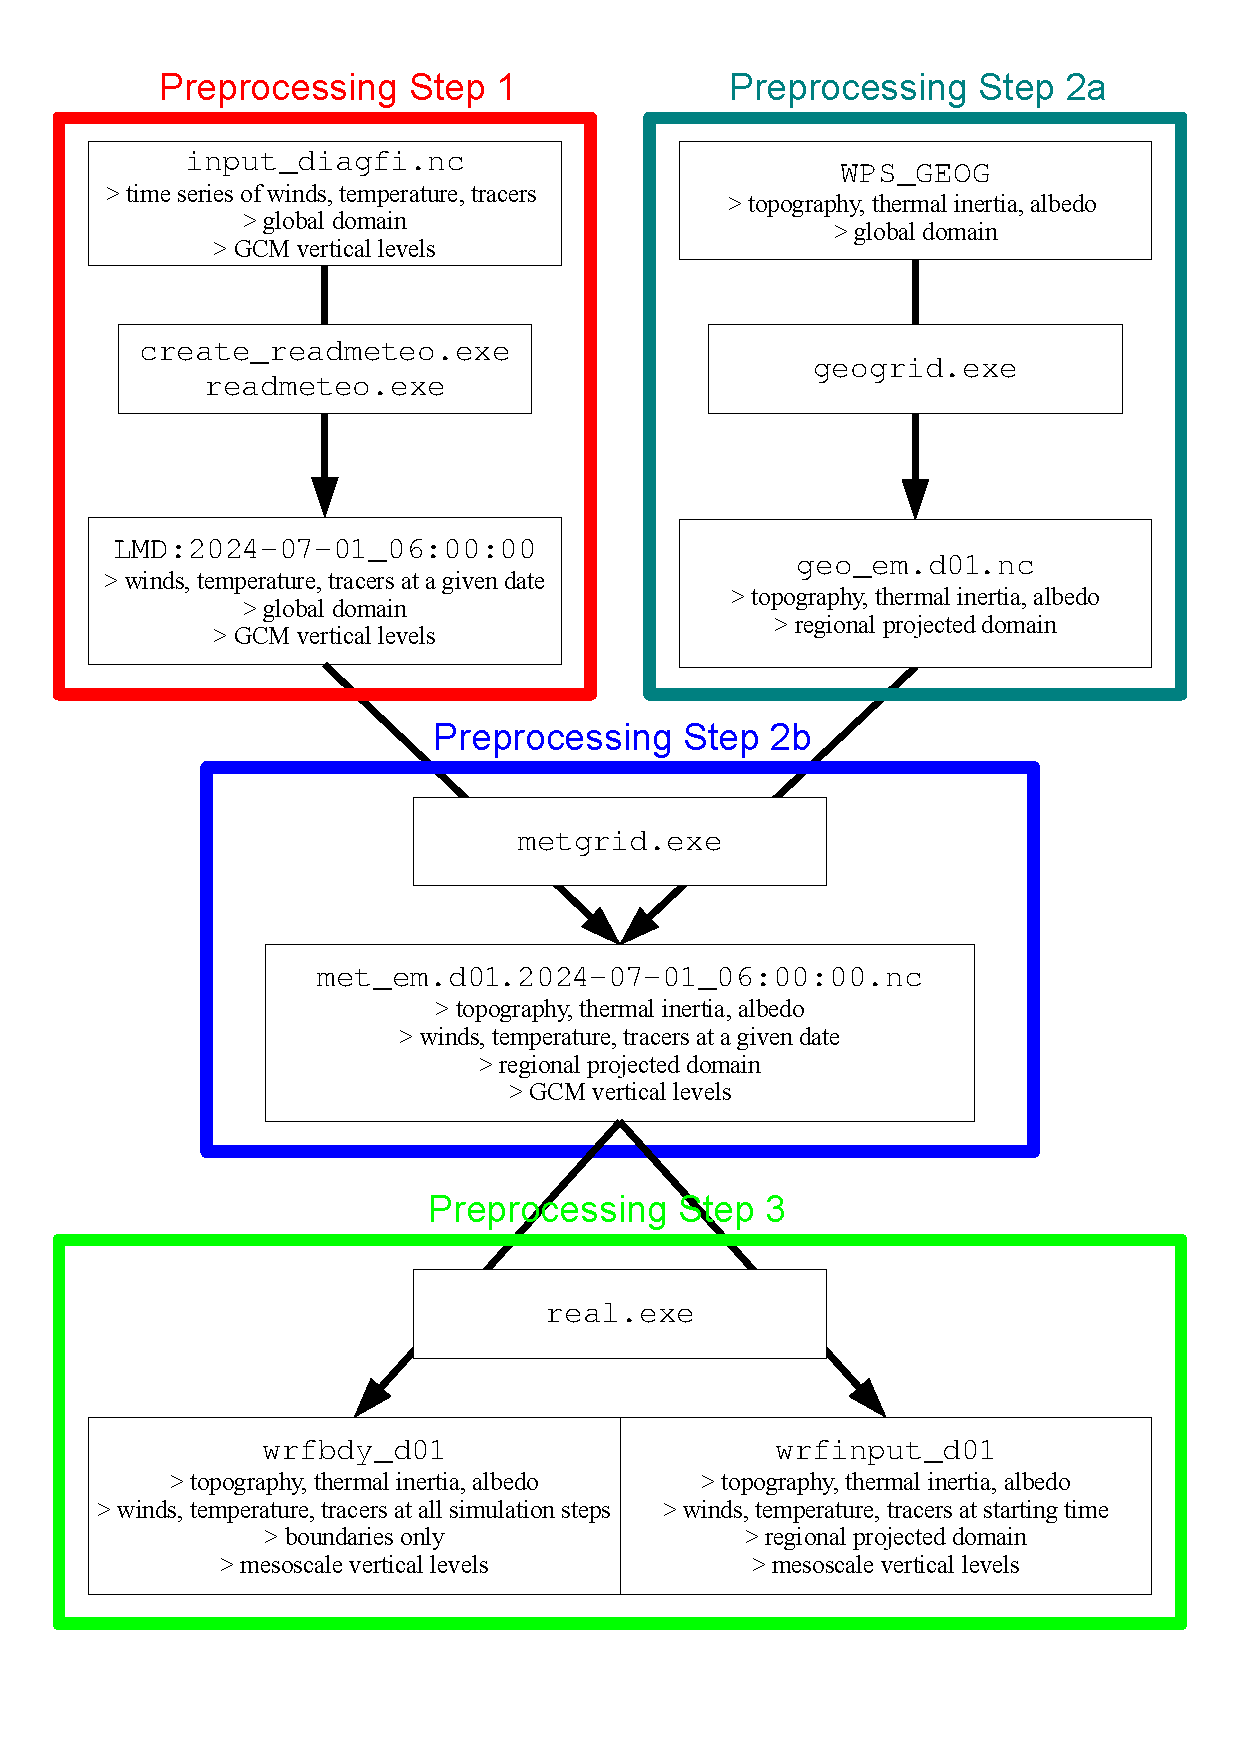
\includegraphics[width=0.99\textwidth]{diagramme.pdf} 
\caption{\label{preproc} The details of preprocessing steps and their related software and inputs/ouputs}
\end{figure}
\end{center}

%\sk
\subsection{Step 1: Running the GCM and converting data}\label{gcmini}

\sk
Here we assume that the user has chosen a given Martian sol or $L_s$ on which to start the mesoscale simulation. As already mentionned in section~\ref{namelist}, the file \ttt{\$MMM/SIMU/calendar} reproduced in appendix can help with this choice (i.e. sol$\rightarrow$$L_s$$\rightarrow$mesoscale date and vice-versa). In addition, the user has to check in the \ttt{calendar} file which sol is before the one wanted for simulation start and has $99$ in the first column: such sols are the ones for which an initial starting file for the GCM is available. Then the number of GCM simulated days \ttt{nday} in \ttt{\$MESO/LMDZ.MARS/myGCM/run.def} must be set accordingly: suppose you want to start a mesoscale simulation at sol~9 during 4~sols, then according to the \ttt{calendar} file, sol~8 is the closest file before sol~9 to be in the database, so \ttt{nday} must be at least~$5$. For optimal forcing at the boundaries, we advise you to write the meteorological fields to the \ttt{diagfi.nc} file at least each two hours, or ideally each hour\footnote{The parameter \ttt{interval\_seconds} in \ttt{namelist.wps} (see section~\ref{wps}) has to be set accordingly.}, i.e. \ttt{ecritphy} is respectively~$80$ or~$40$ in \ttt{\$MESO/LMDZ.MARS/myGCM/run.def}. Eventually the GCM run can be launched using the following commands and should produce a netCDF data file named \ttt{diagfi.nc}:

\begin{verbatim}
cd $MESO/LMDZ.MARS/myGCM
[edit run.def, in particular to modify nday]
./launch_gcm    ## answer: your desired starting sol for the simulations
\end{verbatim}

	%\mk
	%\marge An example of input meteorological file	 
	%\ttt{diagfi.nc} file can be downloaded
	%at \url{http://web.lmd.jussieu.fr/~aslmd/LMD_MM_MARS/diagfi.nc.tar.gz}.
	%%
	%Please deflate the archive and copy the \ttt{diagfi.nc} file
	%in \ttt{\$MESO/TMPDIR/GCMINI}.
	%%
	%Such a file can then be used to define the initial
	%and boundary conditions, and we will go 
	%through the three preprocessing steps.

\sk
Once the GCM simulations are finished, programs in the \ttt{PREP\_MARS} directory allow the user to convert the data from the NETCDF \ttt{diagfi.nc} file into separated binary datafiles\footnote{If the fields \ttt{emis}, \ttt{co2ice}, \ttt{q01}, \ttt{q02}, \ttt{tsoil} are missing in the \ttt{diagfi.nc} file, those are replaced by respective default values $0.95$, $0$, $0$, $0$, tsurf.} for each date contained in \ttt{diagfi.nc} and formatted for the preprocessing programs at step 2. These programs can be executed by the following commands; if everything went well with the conversion, the directory \ttt{\$MESO/TMPDIR/WPSFEED} should contain files named \ttt{LMD:*}. 

\begin{verbatim}
cd $MMM/your_install_dir/PREP_MARS
echo 1 | ./create_readmeteo.exe     # drop the "echo 1 |" if you want control
./readmeteo.exe < readmeteo.def
\end{verbatim}

\sk
\subsection{Step 2: Interpolation on the regional domain}\label{wps}

\sk
\paragraph{Step 2a} In the \ttt{WPS} directory, the \ttt{geogrid.exe} program allows you to define the mesoscale simulation domain, to horizontally interpolate the topography, thermal inertia and albedo fields at the domain resolution and to calculate useful fields such as topographical slopes. Please execute the commands:

\begin{verbatim}
cd $MMM/your_install_dir/WPS
ln -sf $MMM/TESTCASE/namelist.wps .   # test case (or use your customized file)
./geogrid.exe
\end{verbatim}

The result of \ttt{geogrid.exe} -- and thus the definition of the mesoscale domain -- can be checked in the NETCDF file \ttt{geo\_em.d01.nc} e.g. with topographical fields \ttt{HGT\_M} \ttt{HGT\_U} \ttt{HGT\_V} (using for instance \ttt{ncview}, or your favorite graphical interface for netCDF files, or python-based scripts as in section~\ref{postproc}). If you are unhappy with the results or you want to change the location of the mesoscale domain on the planet, the horizontal resolution, the number of grid points \ldots, please modify the parameter file \ttt{namelist.wps}, content thereof is reproduced/commented on the next page\footnote{You may find the corresponding file in \ttt{\$MMM/SIMU/namelist.wps\_example}.}, and execute again \ttt{geogrid.exe}. 

\begin{finger}
\item No input meteorological data are actually needed to execute \ttt{geogrid.exe}. This step~2a can be done e.g. before step~1. It is probably a good idea to prepare step~2 by choosing the mesoscale simulation domain while GCM computations being performed during step~1. 
\item More details about the database and more options of interpolation could be found in the file \ttt{geogrid/GEOGRID.TBL} (for advanced users only).
\item Two examples of \ttt{namelist.wps} parameters are given in Figure~\ref{vallespolar} with resulting domains.
\end{finger}

\footnotesize
\codesource{namelist.wps_example}
\normalsize

\begin{figure}[h!] 
\begin{center}
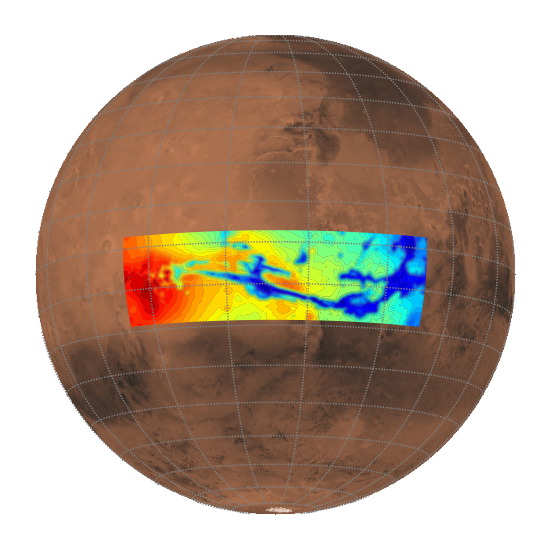
\includegraphics[width=0.48\textwidth]{valles.png}
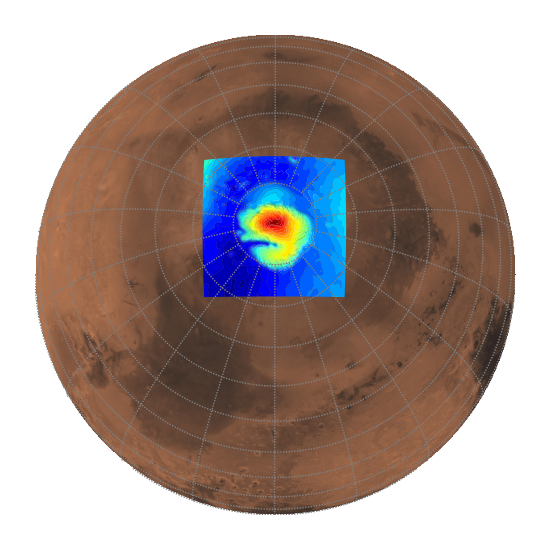
\includegraphics[width=0.48\textwidth]{LMD_MMM_d1_20km_domain_100.png} 
\end{center}
\caption{\label{vallespolar} (Left plot) An example of mercator domain in the Valles Marineris region as simulated by \textit{Spiga and Forget} [2009, their section 3.3]: relevant parameters in \ttt{namelist.wps} are: \ttt{e\_we = 401}, \ttt{e\_we = 121}, \ttt{dx = 12000}, \ttt{dy = 12000}, \ttt{map\_proj = 'mercator'}, \ttt{ref\_lat = -8}, \ttt{ref\_lon = -68}. (Right plot) An example of north polar domain with stereographical projection: relevant parameters in \ttt{namelist.wps} are: \ttt{e\_we = 117}, \ttt{e\_we = 117}, \ttt{dx = 20000}, \ttt{dy = 20000}, \ttt{map\_proj = 'polar'}, \ttt{ref\_lat = 90}, \ttt{ref\_lon = 0.1}, \ttt{truelat1  =  90}, \ttt{stand\_lon =  0.1}.}
\end{figure}

\sk
The input datasets for topography and soil properties can be set in \ttt{namelist.wps} through the keyword \ttt{geog\_data\_res}. Possible choices are:
\begin{citemize}
\item \ttt{'gcm'}: coarse-resolution datasets;
\item \ttt{'32ppd'}: coarse-resolution datasets, but 32ppd MOLA topography;
\item \ttt{'64ppd'}: fine-resolution datasets: TES albedo \& thermal inertia, 64ppd MOLA topography;
\item \ttt{'64ppd\_noHRti'}: fine-resolution datasets, but coarse-resolution thermal inertia;
\item \ttt{'32ppd\_HRalb'}: fine-resolution albedo, coarse-resolution thermal inertia, 32ppd topography.
\end{citemize}
The corresponding dataset must have been built in the \ttt{WPS\_GEOG} folder previously (see section~\ref{wpsgeog}).

\sk
\paragraph{Step 2b} Once the \ttt{geo\_em} file(s) are generated, the \ttt{metgrid.exe} program performs a similar horizontal interpolation of the meteorological fields to the mesoscale domain as the one performed by \ttt{geogrid.exe} for the surface data (interpolation options can be modified by advanced users in \ttt{metgrid/METGRID.TBL}). Then the program writes the results in \ttt{met\_em} files and also collects the static fields and domain parameters included in the \ttt{geo\_em} file(s). If everything went well with the commands below, the directory \ttt{\$MESO/TMPDIR/WRFFEED/current} should contain \ttt{met\_em.*} files.

\begin{verbatim}
cd $MMM/your_install_dir/WPS
mkdir WRFFEED/current
./metgrid.exe
\end{verbatim}

\sk
\subsection{Step 3: Vertical interpolation on mesoscale levels}\label{real.exe}

\sk
The last preprocessing step before being able to run the mesoscale simulation at step~4 is to execute \ttt{real.exe} to perform the interpolation from the vertical levels of the GCM to the vertical levels defined in the mesoscale model. This program also prepares the final initial state for the simulation in files named \ttt{wrfinput} and the boundary conditions in files named \ttt{wrfbdy}. To successfully execute \ttt{real.exe}, you need the \ttt{met\_em.*} files and the \ttt{namelist.input} file to be in the same directory as \ttt{real.exe}. Parameters in \ttt{namelist.input} which controls the behavior of the vertical interpolation are those labelled with \ttt{(p3)} in the detailed list introduced in chapter~\ref{zeparam}. 

\begin{verbatim}
cd $MMM/TESTCASE   ## or anywhere you would like to run the simulation
ln -sf $MESO/TMPDIR/WRFFEED/current/met_em* .
./real.exe
\end{verbatim}

\sk
The final message of the \ttt{real.exe} should claim the success of the processes and you are now ready to launch the integrations of the LMD Martian Mesoscale Model with the \ttt{wrf.exe} command as in section \ref{sc:arsia}.

\sk
\begin{finger}
\item \textbf{ When you modify either \ttt{namelist.wps} or \ttt{namelist.input}, make sure that the common parameters are exactly similar in both files (especially when running nested simulations) otherwise either \ttt{real.exe} or \ttt{wrf.exe} command will exit with an error message. Obviously the dates sent to \ttt{launch\_gcm} and set in both \ttt{namelist.input} and \ttt{namelist.wps} should be consistent too. }
\end{finger}

\clearemptydoublepage

